\chapter{Related Work}
\label{chapter:related.work}

This chapter provides an overview of concepts related to this thesis. We
discuss relevant algorithms in brief and talk about similar projects. In the 
first section we discuss the Paxos family of algorithms and projects in 
this domain in the later sections.

\section{Paxos}
\label{section:paxos}

Paxos is regarded as the simplest and most obvious of distributed algorithms 
\citep{Lamport01}. It is a consensus protocol used for replication of state
machines in an asynchronous environment \citep{Lamport98}. We use Paxos in this
thesis primiarily since it has been shown that it has the minimal possible cost 
of any consensus algorithm in the presence of faults \citep{KeidarR03}.

A consensus algorithm tries to get a group of processes to agree on a value 
while satisfying its safety requirements%
\sidenote{
  Safety requirements of a consensus algorithm \citep{LamportM04}:
  \begin{inparaenum}[(i)]
    \item \emph{Nontriviality}: A value has to be proposed to be choosen.
    \item \emph{Consistency}: Different learners cannot learn different values.
    \item \emph{Conservatism}: Only choosen values can be learned and it can be
      learned atmost once.
  \end{inparaenum}
}. 
These processes in the Paxos algorithm can be classified based on their roles
without affecting its correctness:

\begin{itemize}
  \item \emph{Proposer}: A process that can propose values to the group. 
  \item \emph{Acceptor}: Acceptors form the ``memory'' of the algorithm to 
    allow choosing a single value.
  \item \emph{Learner}: The choosen values are ``learned'' by the other 
    processes.
\end{itemize}

\begin{figure}
  \captionstyle{\raggedright}
  \begin{whole}
    \begin{minipage}[t]{\wholewidth}
      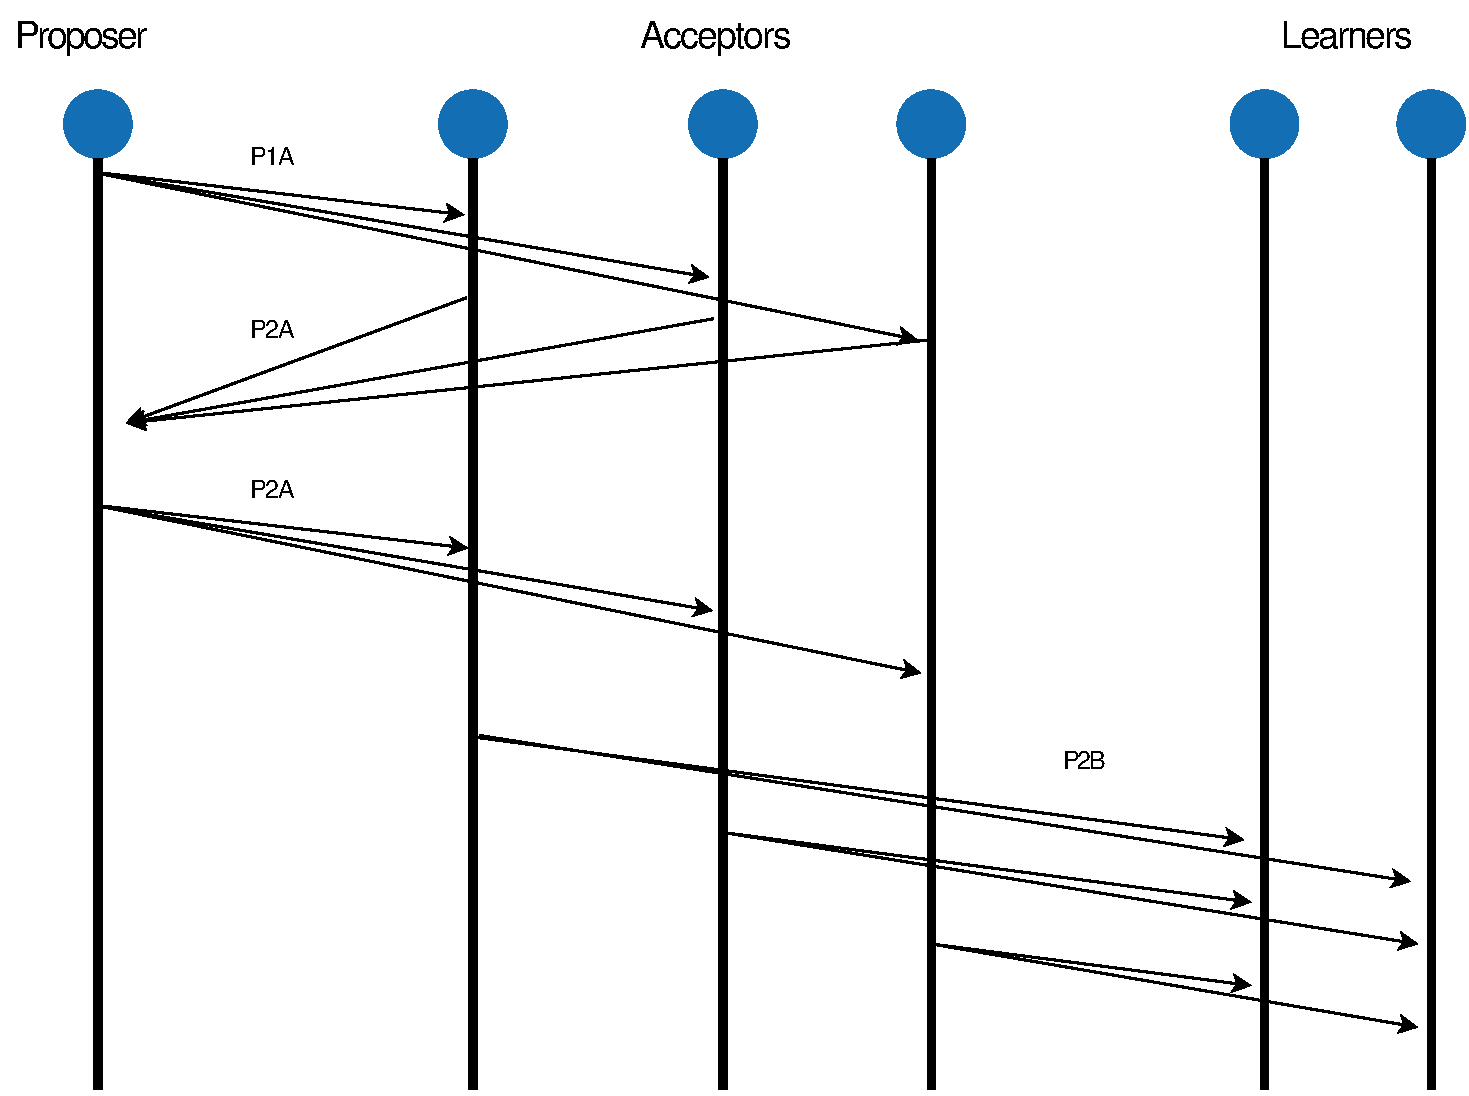
\includegraphics[width=\textwidth]{basic_paxos}
      \caption[Basic Paxos]{%
        Basic Paxos Algorithm: Processes with roles - Proposer, Acceptor, 
        Learner - send messages to each other illustrating the flow of the 
        algorithm in a failure free instance.}
      \label{figure:basic_paxos}
    \end{minipage}
  \end{whole}
  \normalcaption
\end{figure}

The algorithm proceeds in two phases with each phase having two sub phases.

\begin{itemize}
  \iterm{Phase 1 a}: Proposer select a number \emph{n} and sends it as a
  \emph{prepare} (P1A) message to all the acceptors.
  \iterm{Phase 1 b}: Acceptors compares the \emph{prepare} \emph{n} it receives
  and if it is greater than all previous numbers received as a part of 
  \emph{prepare}, it replies (P1B) with a promise not to accept any number lower
  than \emph{n}.
  \iterm{Phase 2 a}: If the proposer receives a response to its \emph{prepare}
  messages from a quorum%
  \sidenote{
    \emph{Quorum}: Majority agreement of processes. Quorum is used to ensure
    liviness in the system.
  }
  , it sends a reply (P2A) back to each of the acceptor with an \emph{accept} 
  message. The message also consists of the value \emph{v} which is the highest 
  numbered proposal among all the responses from the acceptors. In case it is 
  empty, the proposer is free to choose the value.
  \iterm{Phase 2 b}: If the acceptor has not received any \emph{prepare} request
  with a larger number when it receives an \emph{accept} request from the 
  proposer, it sends a message (P2B) to the learner with the accepted value 
  \emph{v}.
  \iterm{Learner}: If the learner receives a message from quorum of acceptor, it
  concludes that the value \emph{v} was choosen.
\end{itemize}

The algorithm makes progress when a proposed value is eventually learned by all
the learners. However, a scenario where no progress is made is possible when we 
have multiple proposers. Consider two proposers issuing \emph{prepare} requests
with alternatively increasing \emph{n}. They would keep pre-empting each other
in a loop leading do no agreement being reached among the group. A solution is
to create the role of \emph{distinguished proposer} or \emph{leader} where it
becomes the only process that can issue new requests. \citet{FisLynPat85}
implies the ``election'' of this \emph{leader} should use either randomness
or timeouts.

Although the pseudo-code of the algorithm is relatively small, implementing it
to create a stable, production ready system is non-trivial \citep{ChandraGR07}.
Different flavours of Paxos allows us to choose specific based on the project's
requirements.

The family of Paxos algorithms differ from each other based on the topology
of the process group, number of phases involved for one instance%
\sidenote{
  An instance of Paxos is a single run of the algorithm starting from the value
  being proposed to the learning of the value by the learners.
}
, amount of message delays and so on. We explore some of these Paxos variants.

\subsection{Basic Paxos}

Basic Paxos is the simplest version of Paxos and is the same as described 
previously in \sectionref{paxos}. The algorithm proceeds over several rounds
with the best case taking two rounds.

\subsection{Multi-Paxos}

The Paxos algorithm needs to be run multiple times for agreeing on a sequence of
values. \emph{Phase 1 a} and \emph{Phase 1 b} of the algorithm become 
an unnecessary overhead if the \emph{distinguished proposer} remains the same 
throught.

Multi-Paxos uses this as its basis to reduce the message flow. The first round 
of Multi-Paxos is the same as Basic Paxos. For subsequent values, the same
proposer starts directly with \emph{Phase 2 a} halving the message complexity.
Another proposer may take over at any point of time by starting with 
\emph{Phase 1 a} overriding the current proposer. This is not a problem since 
the original proposer can start again with \emph{Phase 1 a}.

\citet{Robbert2011} provides the imperative pseudo-code for Multi-Paxos and
the details required for making it practical. This thesis uses this paper as 
its basis for Paxos implementation.

\subsection{Fast Paxos}

Fast Paxos \citep{MSRTR2005112} is a variant of Basic Paxos. It has two
message delays compared to four message delays of Basic Paxos and guarantees
the round in three message delays in case of a collision.

Clients propose the values directly to the \emph{acceptors} and the 
\emph{leader} gets involved only in case there is a collision. Versions of Fast
Paxos can be optimized to a further extent by pre-specifling the collision
resolution technique allowing the clients to fix collisions themselves.

However, according to \citet{Vieira08theperformance} and \citet{Junqueira2007}
Fast Paxos is not better than Basic Paxos in all scenarios. Basic Paxos was 
found to be faster in case of systems with small number of replicas owing to 
the stablility provided by its use of a single co-ordinator and the variation
of message latencies in practical networks. Fast Paxos also needs larger quorum 
sizes of active replicas for it to function.

\subsection{Cheap Paxos}

Basic Paxos requires a total of \emph{2N + 1} servers in a distributed system 
even though \emph{N + 1} servers are enough (minimum) to make progress. 
Using servers that are slower or cheaper for the additional \emph{N} servers
allows us to reduce the total cost of the system. Cheap Paxos is designed along 
these lines.

Cheap Paxos uses \emph{N} auxilary servers along with \emph{N + 1} main servers
which allows it to tolerate \emph{N} failures. The idea is that the auxiliary
server steps to to replace one of the main servers when it goes down 
temporarily. The main server takes back control once restored. The auxiliary
servers thus act as a backup to the main servers without actively taking part
in the protocol, but merely acting as observers.

The downside of using Cheap Paxos is that it affects the liveliness of the 
system when multiple main servers fail at the same time since it takes time
for the auxillary servers to be configured into the system.

\subsection{Ring Paxos}

Ring Paxos \citep{MarandiPSP10} is based on the observations that messaging
using ip-multicast is more scalable and provides better throughput compared
to unicast for a distributed system with a well-defined network. It also
has the property that it provides fixed throughtput with variation in number
of receivers. It claims the throughput of ip-multicast and low latency of
unicast with the downside being that it provides weak synchrony.

\subsection{Stoppable Paxos}

Basic Paxos algorithm is run under the assumption that all the participating
processes are fixed and form a static system. However, the system should
support reconfiguation to be able to run for long periods of time in a
practical implementation. Reconfiguration includes adding new servers, 
removing/replacing old/faulty servers, scaling down the number of servers
when lower throughput is acceptable and so on.

Stoppable Paxos (\citet{LamportSP08}, \citet{LamportMZ10}) is one such algorithm
that allows us to reconfigure a Paxos based system. The algorithm defines a
special set of ``stopping'' commands. A stopping command is issued as the
\emph{i}th command after which no new command \emph{i+1} can be issued. The 
system proceeds normally after it executes the \emph{i}th command.

This thesis uses a variation of Stoppable Paxos for reconfiguration.

\subsection{Other}

Many other flavours of Paxos exists with some of them focussed on the 
implementation aspects of the algorithm. Lets take a look at some of them.

\begin{itemize}
    \iterm{Paxos for system builders}: \citet{Kirsch08paxosfor} provides the
    complete specification for implementing a system based on Paxos. It also
    details the performance, safety and liviness properties of a protoype built.
    \iterm{Paxos Made Live - An Engineering Perspective}: \cite{ChandraGR07}
    details the learning in engineering the Paxos algorithm for use in
    Google Chubby Locks \citep{Burrows06}.
\end{itemize}

\subsection{Implementations}

There are several implementations of Paxos and its variations. We describe full
featured implementations used in production in later sections. We discuss few
Erlang[[]] based implementations below since the thesis project is implemented
in Erlang.

\begin{itemize}
    \iterm{gen\_paxos}: \citep{Uenishi2012} implements Paxos with
    individual processes modelled as finite state machines. Each process can
    be performing a different role based on what state it is on. This 
    essentially makes all processes equal and ready to take on different roles
    as required during runtime.
    \iterm{LibPaxos}: \citet{Lugano2012} is a collection of open source 
    implementations of Paxos created specifically for performance measurements
    in \citet{MarandiPSP10}. It also includes a similator written in Erlang to
    observe the network behaviour.
    \iterm{gen\_leader}: \citet{Ulf2012} implements a leader election algorithm
    not based on Paxos. It is one of the notable implemetations for leader
    election in Erlang.
\end{itemize}

\section{Google chubby locks}

describe chubby locks

paxos made liveA

\section{Google megastore}

\section{Doozerd}

\section{Zookeeper}

this + ZAB

\section{Riak}

\section{Amazon Dynamo}

\section{Dynamo DB}

\section{Scalaris}

